\section{Quantum compilation and intermediate representations}\label{sec:lit_rev:compilation}

Whatever abstractions a quantum programming language offers at its surface, the computation it describes must ultimately be delivered to hardware in an executable form.
This section surveys the compilation stacks that perform that delivery: the shape of their pipelines and the intermediate representations they pass through, the optimisation and resource management performed along the way and the extent to which their transformations can be verified.
The survey ascends the stack, from executable formats through circuit-level optimisation to source-level intent, asking at each level what can be achieved there and what information is missing to go further.

\subsection{Compilation pipelines}\label{subsec:lit_rev:compilation:pipelines}
Compilation pipelines are not specific to quantum programming.
A classical compiler lowers source code through intermediate representations so that transformations independent of the machine are separated from translation specific to it, and a shared representation spares each new language a full compiler for every target.
Quantum stacks adopt the same arrangement, lowering a high-level language through one or more intermediate representations into an executable format consumed by a runtime or hardware controller~\cite{irreview2024}.
Qiskit is a familiar example: a Python framework in which a program constructs a circuit and emits it as OpenQASM~\cite{aleksandrowicz2019qiskit}, a format designed as a hardware-agnostic description of quantum circuits~\cite{cross2017openqasm}.
Emission into such a format does not end compilation.
The emitted circuit may still contain gates the device does not physically implement and refer to qubits by name rather than by location, so decomposition into the native gate set is still required.
Placement of each named qubit onto a physical one under the device's connectivity constraints and realisation of gates as timed control pulses all remain to be performed downstream~\cite{cross2022openqasm3}.
A fully unitary circuit leaves every compilation decision available ahead of execution; hybrid programs remove this guarantee.
A program that measures mid-circuit and feeds the outcome forward into the operations that follow moves part of the pipeline's work into the run itself, so an executable format serving hybrid programs must carry classical control flow alongside gates~\cite{cross2022openqasm3}.

A format in one of these chains can play two roles.
It serves as a terminal target when compilation ends with it and the emitted artefact passes to a runtime unchanged, and as an intermediate representation when further lowering consumes it.
Which role a format plays is fixed by the surrounding stack rather than by anything in the format itself.
OpenQASM is a prolific circuit description language and intermediate representation that takes each role in different pipelines~\cite{cross2022openqasm3}.
Its own specification frames the language both ways, as a description of circuits and as an intermediate representation for compilation~\cite{cross2022openqasm3}.
Recent work on CUDA-Q, a kernel-based programming platform for hybrid quantum-classical computing, treats OpenQASM 3 as an intermediate representation precisely because the format is so widely emitted, ingesting existing programs so they can be compiled onward through its own toolchain~\cite{kulkarni2026openqasm3cudaq}.
The OpenQASM source is parsed into an abstract syntax tree, rebuilt as CUDA-Q kernels and lowered through the compiler framework MLIR into QIR, a quantum extension of the classical LLVM intermediate representation, before any backend is reached~\cite{kulkarni2026openqasm3cudaq}.
Figure~\ref{fig:lit_rev:compilation:openqasm_ambiguity} draws this pipeline alongside the Qiskit stack of the opening paragraphs, in which compilation instead ends at OpenQASM~\cite{aleksandrowicz2019qiskit}.

\begin{figure}[htbp]
    \centering
    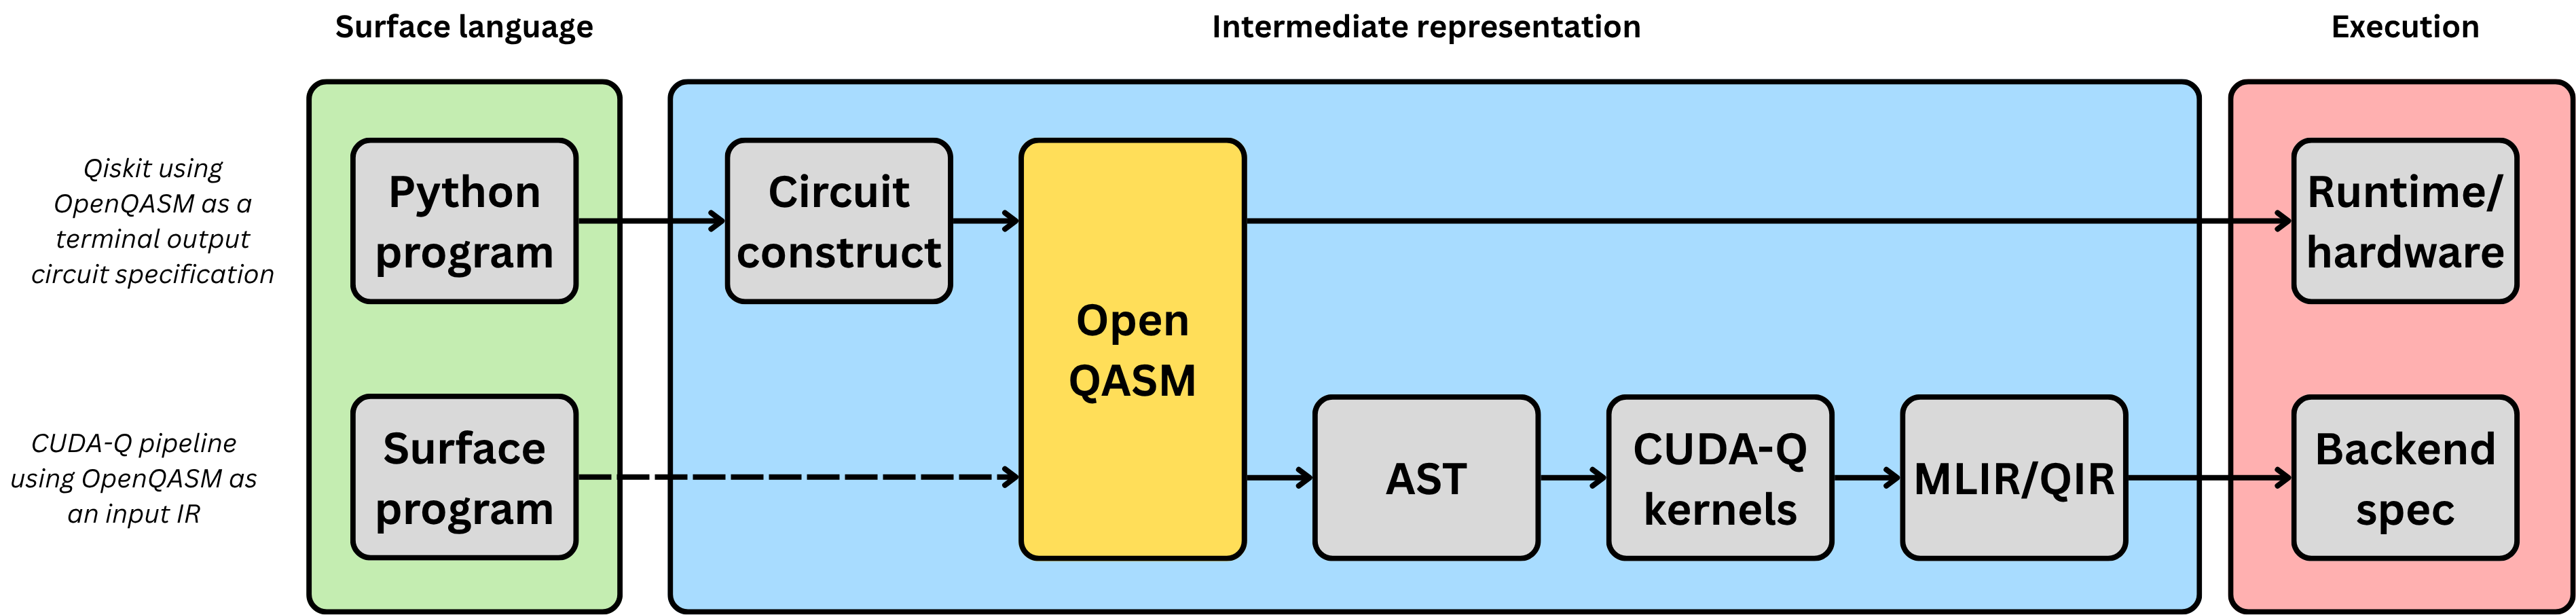
\includegraphics[width=\linewidth]{../figures/fig-lit_rev-compilation-openqasm_ambiguity}
    \caption{OpenQASM is shown as the terminal target of the Qiskit pipeline and as the ingested intermediate representation opening the CUDA-Q lowering chain.}
    \label{fig:lit_rev:compilation:openqasm_ambiguity}
\end{figure}

In both roles the format performs well, and for the same reasons.
A flat sequence of gates over declared registers is concrete, portable across vendors and close to what hardware executes, which is all a terminal target must be~\cite{cross2017openqasm}.
The same flatness serves an intermediate representation provided the analyses asked of it are circuit-shaped; gate sequences admit rewriting, mapping and scheduling directly, which is why lowering pipelines accept them as input~\cite{kulkarni2026openqasm3cudaq}.
What the format bounds is the level of that analysis, because the abstractions that produced the gates were erased at emission.
The boundary is visible even in verified compilation.
VOQC, a machine-checked circuit optimiser, proves that every rewrite it performs preserves the meaning of the gate sequence it receives.
VOQC's guarantees are stated over circuits alone and cannot say whether that sequence realises what the source program intended~\cite{hietala2023voqc}.
A stage below OpenQASM can therefore establish properties of the physical execution but cannot check them against an intent it never saw.
This is a trade rather than a defect.
The format admits the analyses that made it a good target and forecloses the ones that need what emission erased, and the cost of that division to verifying compilation is returned to later in the section.

Whichever role a format plays in these pipelines, what it describes is a circuit.
The circuit model is one of several execution models equivalent up to polynomial overhead, as established in Section~\ref{subsec:lit_rev:quantum_programming:models_of_computation}, yet it is the de facto standard for describing quantum computation.
The prevalence of the circuit model is visible in known quantum intermediate representations; OpenQASM describes circuits by design~\cite{cross2017openqasm}, QIR fixes rules for gates, registers and measurements, and the quantum MLIR dialect that lowers into it defines its operations as register allocation, qubit addressing and gate application~\cite{McCaskey2021MLIRDialectQASM}.
The standard holds because a single circuit-shaped interchange lets any frontend reach any backend, and because gate sequences admit rewrite and equivalence rules simple enough to state and to check mechanically, as VOQC's proofs demonstrate~\cite{hietala2023voqc}.
The same standardisation makes emulation the cost of choosing hardware that realises another execution model; the program is lowered to a circuit as usual and the circuit is translated onto the native model at the final step, so every transformation along the way acts on the emulated circuit rather than on the execution model the machine implements.
The cost lies not in the translation, which equivalence guarantees, but in the optimisations it forecloses.
The same semantic choices in a source program may optimise differently on different execution models, optimising them as a gate sequence no longer describes the intent from which a native realisation could be derived.
In adiabatic computation, an execution model that encodes a computation as the lowest-energy state of a physical system, an emulated gate sequence runs in a time set by the system's spectral gap rather than by its operation count~\cite{aharonov2007adiabatic}.
The gap depends only on the length of the sequence and not on what it computes, so a compiler holding the circuit alone can improve the run only by shortening it~\cite{aharonov2007adiabatic}.
For these processes, optimisation may be better served by a different intermediate representation that encodes computational intent.

\subsection{Circuit optimisation}\label{subsec:lit_rev:compilation:optimisation}
Circuit optimisation rewrites a circuit into an equivalent one that demands less of the hardware executing it.
A quantum processor holds its qubits for a limited time before interaction with the environment degrades them, so a computation must finish inside that decoherence window and every gate it applies is a further opportunity for error.
Shallower circuits fit inside the window and smaller ones accumulate less error, making gate count and circuit depth the base objectives of optimisation.
Fault-tolerant execution shifts the pressure rather than removing it; T gates, whose error-corrected implementation carries a heavy overhead, are costly enough that their count is treated as a resource in its own right~\cite{reducingtcount2019}.
The ZX-calculus is a graphical language that represents a quantum computation as a diagram of connected nodes~\cite{kissinger2019graphtheoreticzx}.
Every circuit converts directly into a ZX diagram, but the calculus is strictly larger than the circuits it contains; its diagrams can be deformed arbitrarily and can pass through intermediate states that no circuit describes~\cite{kissinger2019graphtheoreticzx}.
Figure~\ref{fig:lit_rev:compilation:zx_vs_circuit} contrasts the two representations, showing a circuit alongside the ZX diagram describing the same computation.
That extra space is what makes the calculus effective for simplification; deforming the diagram through states no circuit describes reaches structure that gate-level rewriting cannot~\cite{kissinger2019graphtheoreticzx}.
A general ZX diagram has no guaranteed conversion back into a circuit, so during simplification an invariant called focused gFlow is maintained.
Focused gFlow is a record of the direction in which information flows through the diagram and guarantees that a circuit can be extracted~\cite{kissinger2019graphtheoreticzx}.

\begin{figure}
    \centering
    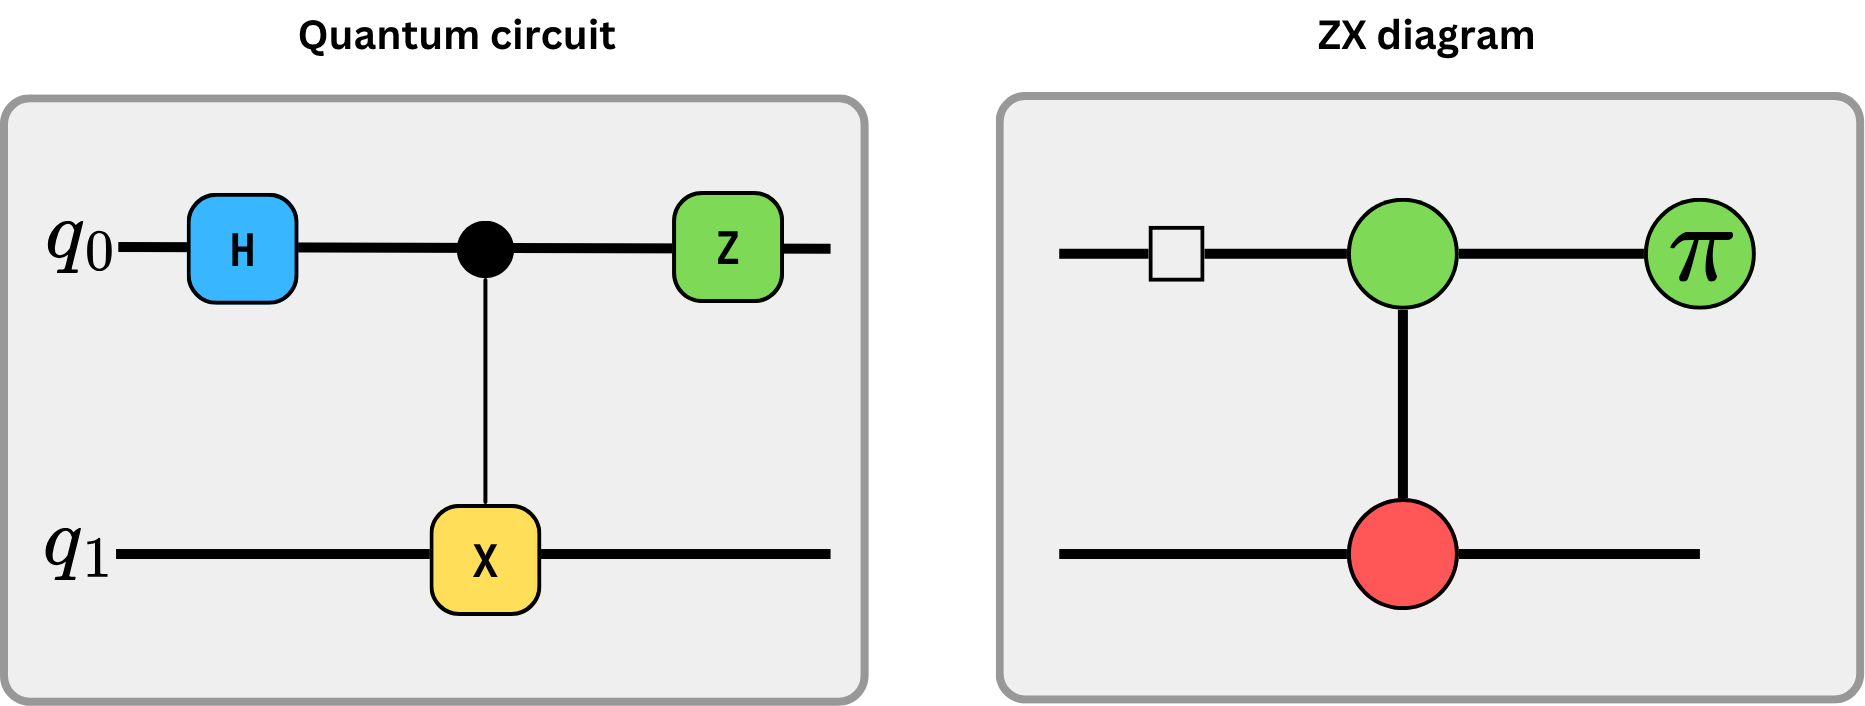
\includegraphics[width=\linewidth]{../figures/fig-lit_rev-compilation-zx_vs_circuit}
    \caption{A quantum circuit and the ZX diagram describing the same computation. Every circuit converts directly into a diagram, while the calculus also admits deformations and intermediate states that no circuit describes.}
    \label{fig:lit_rev:compilation:zx_vs_circuit}
\end{figure}

ZX simplification simplifies the diagram as a whole, a similar approach can be used to achieve targeted T-count reduction~\cite{reducingtcount2019}.
The phases contributed by T gates can be replaced with variables and the diagram simplified symbolically, so that simplification reveals which phases can combine even when their gates sit far apart in the circuit~\cite{reducingtcount2019}.
Unlike diagram simplification the end result indicates which gates of the original circuit can be combined rather than rewriting the circuit or diagram directly.
Circuits with the combinations applied match or improve the prior state of the art on 72\% of standard benchmarks without adding ancilla qubits~\cite{reducingtcount2019}.
VOQC, a verified optimiser, stays inside circuit syntax instead.
It rewrites the gate sequence directly through a library of rewrite rules, each carrying a machine-checked proof that it preserves the circuit's meaning, and achieves comparable reductions in T-count.
VOQC demonstrates verified optimisation is possible~\cite{hietala2023voqc}.
AQCtensor is an approximate compiler for circuits that simulate a physical system evolving in time and optimises classically against that known input structure.
AQCtensor discards standard deep opening circuit structures construction and builds an equivalent, far shallower circuit prefix in its place~\cite{AQCtensor2024}.
As an optimiser it is not generic but demonstrate the utility of manipulating prior semantic knowledge to achieve optimal outcomes, matching the fidelity of the construction it replaces at roughly half the depth~\cite{AQCtensor2024}.

Each of these techniques, generic or specialised, receives a circuit that a programmer has already authored.
Compilation in the general case translates a program from one abstraction to another, and what a compiler can automate is fixed by what its input abstraction makes explicit~\cite{aho2022abstractions}.
A circuit makes explicit how a computation proceeds and nothing of what its values are for.
Continuing to improve optimisations within that limited scope of expression is difficult.
Exact T-count minimisation is exponential in runtime and the practical heuristics improve on it for just 6\% of standard benchmarks~\cite{reducingtcount2019}.
Uncomputation is required wherever ancilla qubits have become entangled with a result, because discarding them unreversed corrupts the measurements that follow~\cite{bichsel2020silq}.
It is also an optimisation opportunity, since uncomputation performed at a convenient point rather than at the site of use shortens the circuit and returns the ancilla for reuse~\cite{paradis2021unqomp}.
Performing it automatically requires knowledge the gate sequence cannot supply, namely which qubits hold temporary values, whether the operations that produced them are classically describable and whether the inputs those operations consumed remain unchanged~\cite{paradis2021unqomp}.
Unqomp, a procedure built to synthesise uncomputation for arbitrary circuits was able to remove 71\% of gates and 19\% of qubits on average from baseline circuit examples in Qiskit by extending it so that ancillae were declared at their allocation~\cite{paradis2021unqomp}.
Silq, a language designed around safe uncomputation, encodes this semantic knowledge in its type system, marking functions as classically describable and their inputs as constant so that every temporary value is guaranteed uncomputable before any circuit exists~\cite{bichsel2020silq}.
What these approaches and those of systems such as AQCtensor demonstrate is that optimisation with semantic knowledge has the capacity to improve on existing state of the art results.

Gate and circuit rewrite techniques converge on closely comparable results regardless of their approach.
Even exhaustive searches of the ZX rewrite space match known heuristic methods on 89\% of benchmarks and never improve on T-count.
The same method improves immediately when redirected at a different objective~\cite{fischbach2025exhaustivesearchzx}.
The equivalent performance demonstrates an upper limit to the optimisation possible with circuit-only context.
In other problem domains improvements were possible by the inclusion of semantic knowledge outside the circuit.
Unqomp demonstrated significant circuit depth and width reductions once ancillae were declared~\cite{paradis2021unqomp} and AQCtensor produced shallower circuits as a  compiler designed around the workload it serves~\cite{AQCtensor2024}.
These kinds of information cannot be recovered by rewrite techniques alone and provide evidence that source expressiveness can provide optimisation gains throughout compilation.